\chapter{Implementation}

%The implementation should look at any issues you encountered as you tried to implement your design. During the work, you might have found that elements of your design were unnecessary or overly complex, perhaps third party libraries were available that simplified some of the functions that you intended to implement. If things were easier in some areas, then how did you adapt your project to take account of your findings?

%It is more likely that things were more complex than you first thought. In particular, were there any problems or difficulties that you found during implementation that you had to address? Did such problems simply delay you or were they more significant? Your implementation might well be described in the same chapter as Problems (see below).

This chapter outlines the process taken to implement this projects, as well as any issues 
encountered during this process and how these issues were overcome. Initially a lot of research
was performed to work out which libraries would suit this project best. A basic framework was then
created following the design in the previous section.

Analysis techniques were then implemented, starting at colour-space analysis and moving up to 
complex texture analysis.

Finally this chapter details the techniques used to classify paintings, from a simple nearest
neighbour algorithm to integrating expert knowledge into the system.

\section{Research into Image Processing Libraries}\label{sec:cv-lib}

Due to the number of libraries out there and lack of experience in the area of computer vision and 
image processing, it was beneficial to research into some of the more popular libraries out there 
to get a feel for each library and image processing in general. This was done by creating a simple
application to perform Gaussian blur on an image, from this it was easy to gauge the use of the 
library and its documentation and could be extrapolated to see how difficult the library in 
question would be to use for more complex applications.

Table~\ref{tab:libraries-overview} shows an overview of all the libraries which were investigated.
Listings can be found in Appendix \ref{sec:code}.

\begin{table}[h]
\begin{tabular}{| c | c | c | c | c | c | c | c |}
								  \hline
\multirow{2}{*}{\textbf{Library}}	& \multicolumn{5}{|c|}{\textbf{Platform}}			& \multirow{2}{*}{\textbf{Language(s)}}	& \textbf{Example}	\\\cline{2-6}
					&  Windows	& Mac 		& Linux 	& Android	& iOS	&			&			\\\hline
\gls{opencv}					& \checkmark	& \checkmark	& \checkmark	& 		& 	& C, C++, Python	& Listing~\ref{lst:opencv}\\\hline
\gls{opencv} - cv2				& \checkmark	& \checkmark	& \checkmark	& \checkmark	& \checkmark & C, C++, Python, Java	& Listing~\ref{lst:cv2}\\\hline
FIJI					& \checkmark	& \checkmark	& \checkmark	& 		&	& Java			& Listing~\ref{lst:fiji}	\\\hline
IVT					& \checkmark	& \checkmark	& \checkmark	& 		&	& C++			& Listing~\ref{lst:ivt}	\\\hline
\end{tabular}
\caption{Comparison of image processing/computer vision libraries.}
\label{tab:libraries-overview}
\end{table}

\gls{opencv} appeared to be the most polished of all the libraries researched into, boasting a 
wide range of features with comprehensive documentation, especially for \gls{cv2}, which, as has
previously been discussed, is the more recent version of \gls{opencv}. 

\gls{fiji} has a good range of high-level features, especially through their GUI elements, however
for use as a library it was rather unwieldy and difficult to find the classes which performed 
simple functionality. Combined with equally bad documentation it was already unlikely to be used
but when, after fifteen minutes of struggling with the API images could only be blurred into a
grey-scale output, it was completely discounted.

It should be noted that most of the \gls{fiji} features weren't used at all and the actual code
seemed to just use ImageJ libraries. \Gls{fiji} is often descibed as a distribution of 
ImageJ\cite{Schindelin2012Fiji}, the analogy ``As Ubuntu is a distribution of Linux, \gls{fiji} is a 
distribution of ImageJ'' is commonly used to describe this further.

To continue that analogy, when programming with operating system libraries; it is common only to 
use the core libraries; not those libraries made to use the kernel more usable. The same logic
applies with \gls{fiji} and ImageJ; whilst \gls{fiji} provides a cleaner interface in which to use
the libraries, at its core it is still calling ImageJ methods. On reflection it would have been 
better to only consider ImageJ rather than the more cluttered \gls{fiji}.


\gls{ivt} was somewhat similar to \gls{fiji} in that it had a good range of high-level features, 
but was less impressive as a library. Even following the example code it was difficult to 
compile against \gls{ivt}, despite using the makefiles provided in their own examples.

It was, therefore, an simple choice with only one library being workable for this project. Not only
was \gls{opencv} the top choice from the above research, it is also one of the most prevalent
libraries for computer vision problems.

Later in the project, the transition was made to \gls{cv2}, therefore it has been added to the
above research for completeness. When comparing \gls{opencv} and \gls{cv2} it is apparent that
\gls{cv2} is much easier to work with and also has much better documentation.

\section{Basic Structure}

\subsection{Loading Data}
One of the more key parts to implement before all others in this project is the ability to load in
data from the initial spreadsheet. The first step of this was to convert it to a \gls{csv} 
file-type, which is easier to read programatically.

Initially the spreadsheet has a different format from the version depicted below. In this version 
the file names tended to be much longer and were in sub-folders depending on their collection. 
Extra logic was needed to locate the file, though this was a simple matter of concatenating the 
collection to the file name as a directory. 

Later in the project a new version was provided by Lloyd, the format of which is shown in Table~
\ref{tab:spreadsheet-format}, this was then converted to a \gls{csv} file format shown in Figure~
\ref{fig:csv-spreadsheet}. This makes the spreadsheet data easier to parse digitally as there are
many libraries available to parse \gls{csv} files whereas attempting to parse a specialised 
spreadsheet format. This was also a good excuse to clean up some of the initial code to 
use better Python programming practises; replacing messy loops with list comprehension where 
possible, using \gls{kwargs} and dictionaries instead of having utility methods, etc.

\begin{table}[h]
\resizebox{\textwidth}{!}{
\begin{tabular}{|c|c|c|c|c|c|c|c|c|c|c|c|c|} \hline
Filename & ID & Title & Catalogue entry BBC YP & Genre & Height & Width & Area & Materials & 
Collection & image width & image height & image height/image width \\ \hline
001.jpg & 1 & A Chapel in the Tyrol & 1950-1960 & Landscape & 40.7 & 29.8 & 1212.86 & oil on 
hardboard & NLW & 687 & 944 & 1.3741 \\ \hline
\end{tabular}
}
\caption{Layout of the Painting Data Spreadsheet}\label{tab:spreadsheet-format}
\end{table}

\begin{figure}[h]
\resizebox{\textwidth}{!}{
\texttt{001.jpg,1,A Chapel in the Tyrol,1950-1960,Landscape,40.7,29.8,1212.86,oil on hardboard,
NLW,687,944,1.3741}
}
\caption{Painting Data in CSV Format}\label{fig:csv-spreadsheet}
\end{figure}

This \gls{csv} file was then parsed using the Python 2.7 in-built \texttt{csv} module with 
relative ease. The example code (see listing~\ref{lst:csv_example_code}) helped to ensure correct
resource management as well as showing how the library parsed files.


\subsection{Top-Level Classes}
This section focuses on implementing code based on the design shown in Figure~\ref{fig:uml-final}.
Being used to Java, the initial instinct was to set up interfaces for the majority of 
top-level classes (namely the \texttt{Analyser} and \texttt{Classifier} classes). However, 
Python does not have the concept of interfaces, so normal classes were used to represent these
instead. These classes acted as abstract stub classes and just held place-holder method definitions
which needed to be overridden in the concrete sub-classes. This was a slightly pointless exercise 
due to the duck typing, but was useful to depict the architecture in code. It also became more 
useful when these classes began to define a lot of the common methods.

A \texttt{Painting} class was also implemented and had a builder method to take an array (from the
\gls{csv} file) and create a new instance of it from this. Later this was changed to make use 
Python \gls{kwargs} instead to make it easier to both read and process, especially in the exemplar
work where mock objects were used.


\subsection{Command Line Interface}
As a research program with lots of different analysis and classification techniques the next step
in setting up the basic architecture was to create a set of command-line arguments which would
switch the functionality of the program. These arguments are depicted in Table~\ref{tab:args}.

\begin{table}[h]
\centering
\begin{tabular}{|c|c|c|c|} \hline
Name             & Short Flag & Long Flag         & Description\\\hline
Analyser         & \verb+-a+  & \verb+--analyser  +& Switch the analysis technique\\
Machine Learning & \verb+-m+  & \verb+--ml        +& Switch the machine learning technique\\
Data             & \verb+-d+  & \verb+--csv       +& The data file to use\\
GUI              & \verb+-g+  & \verb+--gui       +& Switch the GUI visualisation\\
Binning          & \verb+-5+  & \verb+--bin-years +& Round paintings to the nearest 5\textsuperscript{th} year\\
Export           & \verb+-e+  & \verb+--export    +& Export analysed data\\
Classify         & \verb+-c+  & \verb+--classify  +& Classify the specified image\\
\hline
\end{tabular}
\caption{Command Line Arguments}\label{tab:args}
\end{table}

The \texttt{argparse} library handles this nicely, the example code shown in 
listing~\ref{lst:argparse_example_code} shows the usage of this library.

These flags then hook into the factory methods to actually create the instances and return them to
the central point which then called them where required. A 
fa\c{c}ade\cite[p.185-194]{Gamma1996Design} was used to hold and call these instances, as well as
handling the calls to the factories.


\section{Colour Space Analysis}
Colour space analysis involves performing statistical analysis on different colour models 
(\gls{rgb}, \gls{hsv}, etc.). This gives a very simplistic view of the entire image, through 
creating a small histogram representing mean colour over the entire image.

\gls{opencv} offers a method to perform the average across the image, however with a
further look into the documentation there is also a method which performs both 
mean and standard deviation on an image.

The analysed data was just the tuple returned by this method. The distance measure
was defined to be the sum of all elements in the tuple (in the case of an \gls{rgb} colour model
the mean red, green and blue and the standard deviation of red, green and blue).

\subsection{Colour Models}
There are many colour models to consider with digital image processing. \Gls{rgb} is one of the
better know colour spaces as it is often how images are captured. It does have a feature in that
all three values can change when the brightness changes.

As one of the main hypotheses of this project is that Williams' work darkened over time, it
may follow that \gls{rgb} may not be the best colour model to use.

To account for this it was decided to also use a \gls{hsv} colour model to compare and contrast 
\gls{rgb}. \Gls{rgb} is a colour-model in which a pixel of colour is represented by three 8-bit
values, one for the intensity of each colour. \Gls{hsv}, in contrast, is a colour model which uses
a range of $360^\circ$ for the hue and is the only representation of colour in this model. The 
value defines the lightness of the colour and the saturation defines the degree to which the 
colour is present.

\gls{opencv} handles colour spaces slightly oddly. Initially it uses a method to load the 
image, which uses an integer argument as a flag to define whether the image should be loaded in 
colour or grey-scale.

From this image you then can use a function to convert the colour model of an image, which 
uses an integer argument as a flag to define a number of different colour spaces.
Once converted, all methods act exactly the same as they would on a \gls{rgb} image.


\subsection{Colour Histograms}
Colour Histograms are a representation of the distribution of colour across an image; this makes
them very powerful for analysing the colour space of an image. For digital images, histograms are
the number of pixels which have a colour in a fixed range of colours. These ranges are typically
referred to as the bins of a histogram. These bins are arranged so they span the range of colours
in the entire colour space.

\gls{opencv} provides a number of methods for both calculating and operating upon colour histograms. 
Here the example code (Figure~\ref{lst:opencv_histogram}) from the \gls{opencv} documentation was a
useful reference as some of the details of creating histograms in \gls{opencv} are not noted explicitly
in the python documentation.

Initially this was performed as a 3D histogram to span three channels of the chosen colour model 
representation; for an \gls{rgb} representation each dimension represents one of the three primary
colours - red, green and blue. A low number of bins was also used to keep the memory limits down
as this was a very large object if the whole range of colour in the model are represented.
Later on, with the move to \gls{cv2}, this became a less expensive option and it was possible to
create a 2D histogram for each channel in the colour model.

The distance measure between colour histograms is also handled by \gls{opencv} using a compare histogram
method. Under the covers this uses a \gls{chi2} (Equation~\ref{eq:chi_squared}) method to
compare to histograms of equal dimensions. \gls{chi2} is not the only distance measure that can be
applied to histograms; distance measures like Euclidean and Manhattan distance which have been 
previously mentioned can also be applied to histograms, but do not include normalisation that 
\gls{chi2} does so they are less useful to the histograms used in this project.

\begin{equation}\label{eq:chi_squared}
\chi^2(H_1,H_2) =\sum_I{\frac{(H_1(I) - H_2(I))^2}{H_1(I)}}
\end{equation}

There are other methods of comparing histograms to one another, which \gls{opencv} provides by 
default, but which are not very well suited to the application. Methods like histogram 
intersection where, for each bin, the smallest value is chosen between the two histograms; or 
calculating the correlation between two histograms, are obviously less useful than an actual 
measure of distance.


\section{Texture Analysis}

\subsection{Edge Count}
The simplest technique to analyse texture is to apply an edge detection algorithm over the image
and produce a count of all the marked edges regardless of orientation.

The Canny edge detector\cite{Canny1986Computational} provided a good output for measuring this, 
operators like Sobel provided less useful results and thus provided a worse analysis technique.

From the generated image a histogram was produced with only 2 bins; one bin for the presence of an
edge, the other for the absence of an edge. The second bin is just to help with the normalisation
of distances as it is just the number of pixels in an image minus the number of pixels in bin one.

Open CV provides methods for applying the Canny edge detector to an image so this technique was 
simple to implement.

%TODO Image of the Canny'd image.

\subsection{Histograms of Orientation Gradients}
This technique is based on the \gls{hog} paper\cite{Dalal2005Histograms} and mirrors some of the
implementation in a simplified fashion.

The main crux of the method was to generate the exact orientation of a given point of an image,
apply this across the image and then bin the results into a histogram. The original paper then
focused on using this for human recognition and aimed to keep the time complexity down through
normalisation, applying it to this project only needed the generation of the histogram of exact
orientations.

Calculating the edge orientation involves passing a filter over an image which is used to find the
orientation of that gradient. 

There are many forms of filter which can be used to do this. The simplest of which discrete 
derivative masks, steerable filters 
are a more adjustable implementation of this. There are also more complex filters, like Gabor 
filters, which provide better flexibility and matching.

Using discrete derivative masks it is fairly simple to work out to orientation of a gradient 
mathematically. First pass a mask of the form $\left[\begin{smallmatrix}-1\\0\\1\end{smallmatrix}\right]$, followed
by one in the form $\left[\begin{smallmatrix}-1 & 0 & 1\end{smallmatrix}\right]$. These give 
$\frac{\delta f}{\delta x}$ and $\frac{\delta f}{\delta y}$ respectively.

A gradient direction function, shown in Equation~\ref{eq:grad_dir}, can then be used on both these
values to work out the actual direction of the gradient.

\begin{equation} \label{eq:grad_dir}
\theta = {\rm atan2}\left( \frac{\delta f}{\delta x}, \frac{\delta f}{\delta y} \right)
\end{equation}

\subsubsection{Caching of Histogram of Orientated Gradient Results}\label{sec:hog-canning}
Working out the exact orientation of a gradient is a costly operation and it became useful to
\emph{cache} (persist) the results to allow the technique to complete in a decent amount of time.
This change was made after the change to \gls{cv2} and was done using numpy methods for
simplicity. 

For speed of execution and in order to experiment with bin sizes it was easier to cache the 
results from the gradient direction function than to just cache the final histogram result. This
allows for the ease of comparison between all forms of texture analysis.

\subsection{Steerable Filters}
Another way of analysing the distribution of edge orientations to change the orientation of the filter and bin the direction into 
certain cardinal directions; typically $0$, $\frac{\pi}{4}$, $\frac{\pi}{2}$ and $\frac{3\pi}{4}$
(from $\pi$ to $2\pi$ becomes a repeat of any of those directions, only in reverse and are, 
therefore, covered already).

To do this steerable filters $S(\theta)$ can be used (shown in Figure~\ref{fig:steerable-filters}). 
The angle of the filter ($\theta$) is manipulated to match the four cardinal directions, which 
will then give the degree to which a gradient matches that angle. A histogram is created with a
bin for each value of $\theta$, these bins are added to if the value of a given filtered pixel is
above a threshold, helping to prevent the overlapping of orientations.

\begin{figure}[h]
$$
S\left(0\right) = 
\begin{bmatrix}
0 & 1 & 0 \\
0 & 1 & 0 \\
0 & 1 & 0
\end{bmatrix}
S\left(\frac{\pi}{4}\right) =
\begin{bmatrix}
0 & 0 & 1 \\
0 & 1 & 0 \\
1 & 0 & 0
\end{bmatrix}
S\left(\frac{\pi}{2}\right) = 
\begin{bmatrix}
0 & 0 & 0 \\
1 & 1 & 1 \\
0 & 0 & 0
\end{bmatrix}
S\left(\frac{3\pi}{4}\right) = 
\begin{bmatrix}
1 & 0 & 0 \\
0 & 1 & 0 \\
0 & 0 & 1
\end{bmatrix}
$$
\caption{Steerable Filters}
\label{fig:steerable-filters}
\end{figure}

These have the advantage of being far less complex to compute than edge orientation; the maths and
histogram creation on a floating point array are costly operations, to the point where
canning the results for edge orientation is desirable.

There is the obvious trade off that steerable filters can only work in four directions which
does affect the performance quite severely.

\subsection{Gabor Filters}
To increase the orientations matched from steerable filters without the need for increasingly 
large kernels, Gabor filters\cite{Daugman1985Uncertainty} were implemented. Gabor filters allow
for an almost-infinite range of orientations without affecting the size of the filter. To do this
they use a sinusoidal wave; which matches gradients, wrapped in a Gaussian envelope. Figure~\ref{fig:gabor}
shows an example Gabor filter and Equation \ref{eq:gabor} shows the mathematics used to generate a Gabor Filter.

\begin{figure}[h]
\centering
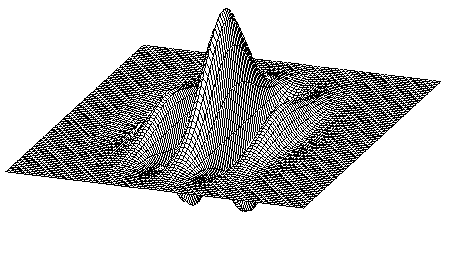
\includegraphics[width=0.5\textwidth]{img/gabor-real}
\caption{The real part of the impulse response of a Gabor filter\cite{Trapp1998Gabor}}\label{fig:gabor}
\end{figure}

\begin{align}\label{eq:gabor}
g(x, y; \lambda, \theta, \psi, \sigma, \gamma) &= \exp \left( -\frac{x'^2+\gamma^2y'^2}{2\sigma^2} \right) \cos \left( 2\pi \frac{x'}{\lambda} + \psi \right)
\intertext{where:}
x' &= x \cos \theta + y \sin \theta \nonumber \\
y' &= x \sin \theta + y \cos \theta \nonumber
\end{align}

As with steerable filters the convolution of an image with a set of Gabor filters were accumulated in a histogram. Initially Gabor
filters were implemented with the same 4 orientations as steerable filters ($0$, $\frac{\pi}{4}$,
$\frac{\pi}{2}$ and $\frac{3\pi}{4}$), however this has the problem that the variation in orientations is not being utilised.

To solve this issue the way Gabor filters were initialised was changed by adding in a 
parameter which defined the number of orientations that instance of the Gabor filter would have,
the logic of which is defined in Figure~\ref{fig:gabor-init}, note that the range is $1\dots b$,
as $\theta=0$ and $\theta=\pi$ will produce the same result (both matching vertical lines best).
This helps to prevent certain mathematical issues, particularly those involving passing $\theta$
in as 0.

\begin{figure}[h]
\begin{algorithmic}
\Function{Gabor.init}{$b$} \Comment{$b$ is the number of orientations}
\For {$i \in 1\dots b$}
\State $\theta_i \gets \frac{i\pi}{b}$ \Comment{$\theta$ is the list of orientations to produce filters for}
\EndFor
\EndFunction
\end{algorithmic}
\caption[Psuedocode for Gabor Filter initialisation]{Psuedocode for Gabor Filter initialisation including number of orientations to produce 
filters for}\label{fig:gabor-init}
\end{figure}

The actual Gabor filters are then produced for all values in $\theta$ at runtime and applied to
the images in turn.

An example section of MATLAB code which implements Gabor filters shown in Listings~\ref{lst:gabor}
\cite{Yang2010Gabor} was used as a reference to write the code for the Gabor filters. This code
was improved to make use of numpy array manipulation functionality as well as to be more readable.


\section{Brush-Stroke Analysis}

Due to time constraints it was not viable to look at brush-stroke analysis, especially with the
shift of focus to exemplars after texture analysis.

It would have been nice to explore this area due to Williams' style, but a lack of high-resolution
images would have also made this a difficult area to get right.

There were several good ideas thought of for this area. One was to train a machine learning 
technique to recognise brush-strokes through the manual marking of strokes. This would have been a
very interesting method to try, especially being able to apply existing techniques to aid and
improve the classification of brush-strokes.

Other techniques involved passing filters over the image looking for the edges of brush-strokes
\cite{Berezhnoy2009Automatic}, then applying other operations to complete the stroke area. This
is a much simpler technique which will likely give bad results due to the low resolution and
non-uniform scaling of the images as it seems to be very dependant on the filter.

One final technique suggested by Li et al.\cite{Li2012Rhythmic} involves a combination of edge
analysis and clustering in colour space with a number of heuristics involving branching, 
stroke-width modelling and gap filling to refine the original brush-stroke estimates.

The difficulty that would be associated with this section of work is that existing techniques may
not be applicable to Williams' work due to his use of the palette knife. Whilst there are very
obviously clear strokes in his work, comparing these strokes to the likes of Van Gogh are unlikely
to pay off due to the \emph{blockier} strokes of the palette knife this is another reason this analysis
technique was side-lined in favour of exemplars.


\section{Ensemble Methods}
Ensemble methods are commonly used in statistical and machine learning to improve the performance,
the main concept of an ensemble method is to combine two or more models to produce better results
than would be gained from a single model.

The simplest form of ensemble methods just involve running all models in the ensemble, combining them into
one large histogram and then performs normal distance measure on them. However, due to some 
problems with the \gls{cv2} histogram calculation method, it was a lot easier to flatten
(to collapse a multi-dimensional array into a one-dimensional array) the results from each 
analysis technique making up the ensemble method.

This does affect the performance a little, but it is better than the other solution of adding 
resulting distance from each model together as the distances are not normalised. This was my 
initial solution to the problem and hugely affected the results as the distance returned from
statistical colour-space methods is a lot less than those returned from colour histograms and so
on.

Of course it would also be possible to normalise each distance measure of each technique, but this
would be difficult as the mean and variance of the distance for an analysis technique is not 
tracked. It may also cause problems when new examples are added (during validation, for example)
which affect both these values.

This method is commonly known as \gls{bagging}; where each model has a ``vote'' with equal weight.

One part I considered adding to this, but didn't have the time to complete, would be to weight the
vote of each technique (likely via a machine learning technique) in the ensemble so that the 
better performing techniques affect the results more.

Another method commonly used in machine learning is Boosting, where the model is built 
incrementally, with the focus being on examples which were mis-classified by the previous models.
This method does improve accuracy, but is known to over-fit the dataset. 


\section{Classification and Validation}
With the results of analysis techniques there's also a need to be able to classify paintings based
on these results and also to validate the results of both so that different methods of analysis
and classification can be compared for performance.

\subsection{$k$-Nearest Neighbour}
The simplest method of classification is to work out which painting in the dataset is closest in
feature space to the painting which needs to be classified and classify the year of this painting
with the year of the nearest painting.

This is a Nearest Neighbour algorithm with $k=1$, Figure~\ref{fig:1nn} shows the psuedocode
for this algorithm

\begin{figure}[h]
\begin{algorithmic}
\Function{1-NN}{$p$, $data$}
\State $n = \operatorname*{arg\,min}_{d \in data}$ \Call{Distance}{$p, d$}
\State\Return $n_{year}$
\EndFunction
\end{algorithmic}
\caption{Psuedocode for 1-Nearest Neighbour}\label{fig:1nn}
\end{figure}

From 1-Nearest Neighbour it is a simple matter to change this to a $k$-Nearest Neighbour algorithm
as Figure~\ref{fig:knn} shows.

\begin{figure}[h]
\begin{algorithmic}
\Function{k-NN}{$p$, $data$, $k$}
\ForAll {$k$}
\State $n = \operatorname*{arg\,min}_{d \in data}$ \Call{Distance}{$p, d$}
\State $a \gets a + n_{year}$
\State $data \gets data \setminus n$
\EndFor
\State \Return \Call{Average}{$a$}
\EndFunction
\end{algorithmic}
\caption{Psuedocode for $k$-Nearest Neighbour}\label{fig:knn}
\end{figure}

With this, the method of averaging the year can be any statistical method of taking the average
(mean, median or mode). Mean is the typical case for $k$-Nearest Neighbour as it is simple to
implement. Median is less common as it is slightly more complex to implement. Mode is more 
difficult to implement programmatically, especially given the sparseness of the data. 

However, using mean raises an interesting problem. Mean returns a point, in this case a year, 
which may not be a year of any painting in the dataset. Median and mode will nearly always return
a year in the dataset. With mean there is an implicit assumption that Williams painted every year
without a gap whilst our dataset does have these gaps. 


\subsection{Leave-One-Out Cross Validation}
To validate the classified years from $k$-Nearest Neighbour, this project uses Leave-one-out Cross
Validation; a technique which involves removing each point from the known dataset, applying the
classification technique to this point against the remaining dataset. This produces a list of
classified years against the actual years.

To measure the goodness of fit the Pearson's product-moment correlation coefficient was 
calculated on these orderings; this provides us with a performance measure of each classifier. 
It is also possible to test Pearson's R for statistical significance.

Correlation is the measure of statistical relationship between two sets of data, a correlation of
$1$ is a perfect match where one set of data is exactly equal to the other. A correlation of $0$
means there is no identifiable match between the datasets and a correlation of $-1$ is where the
datasets are opposite to one another. Because the aim is to have the classified exactly equal to
the actual year, a correlation closer to $1$ means that the classified years are closer as a whole
to the actual years.

Another measure applied alongside correlation is statistical significance. This is the degree to
which a statistical result could have occurred by chance given a null hypothesis. This can be applied
to a correlation to calculate the extent to which the correlation could have been arrived at by 
chance.

Overall it is best to try and maximise the correlation between two data-sets whilst keeping the
significance low. Pearson's product-moment correlation is able to generate the correlation between
two data-sets and also defines a method of generating the statistical significance on top of this.
numpy's implementation of this provides both the correlation and p-value (significance) as part of
the return value.

Both of these are easy to implement - leave-one-out cross validation just involves iterating over
the entire list of known paintings, popping the current painting from the list and running the 
classifier on it, then pushing it back into the list at its original position.

A plotting library, matplotlib, was used to generate scatter plots of actual year against 
classified year to represent this data visually. An example of this is shown in Figure~\ref{fig:scatter}

\begin{figure}[h]
\centering
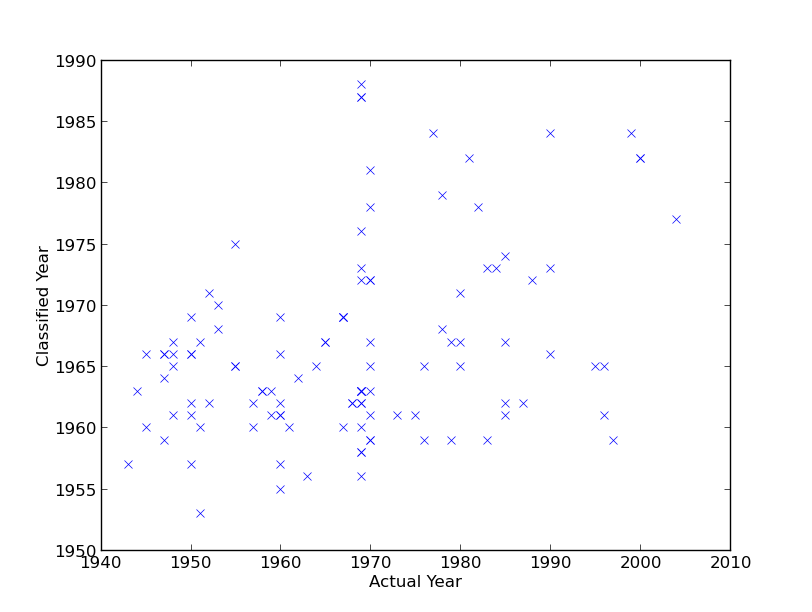
\includegraphics[width=0.75\textwidth]{img/scatter.png}
\caption{Scatter Plot of Actual Year against Classified Year for Gabor Filters and $k$-Nearest 
Neighbour ($k=7$)}\label{fig:scatter}
\end{figure}

\subsection{Weka 3}
Weka is a collection of machine learning algorithms\cite{Hall2009WEKA}, used predominately for
data mining. Due to the number of machine learning techniques it provides, it was interesting to
input data from the analysis techniques into Weka.

The first classification technique applied through Weka was linear 
regression\cite[p.717-727]{Russell2010Artificial}: the act of fitting a linear function to the 
training data-set then classifying new examples using this function. The function can either be
univariate (a straight line function) or multivariate, where each example is an $n$-element 
vector. For our data multivariate is more applicable but may require a reduction in the complexity
of the function to avoid the overfiting of data (where the classifier is to specific to the 
training data-set and cannot generalise to new examples well).

Another set of classifiers applied to the data-set through Weka were artificial neural 
networks\cite[p.727-737]{Russell2010Artificial}. Neural networks are biologically inspired 
classifiers which use layers of nodes or units, which are connected with directed links. The 
simplest form of neural network, a single-layer feed-forward neural network (preceptron), where
all input nodes are connected directly to outputs was used. As well as a more complex neural 
network with a set number of hidden layers - layers of nodes which do not directly correspond to
the inputs or outputs, but which perform some intermediary function.

Unfortunately, it seems that the data provided to Weka is not well suited to most of the methods 
in the tool-kit. The data was, perhaps unsurprisingly, ill suited to regression techniques; each
parameter has such a variable set of values that it is difficult to perform regression on these
parameters.

Similarly, Neural Networks also perform badly, again it seems that so many of the parameters can
take on such widely different values, even in the same year group, that it is difficult to build
a model to suit the data.

In the end Weka proved to be more time consuming than it was worth and, though it did provide a 
few interesting results, the variation in data proved just too much for it.

$k$-Nearest Neighbour does not suffer from this flaw as it does not need to build a model based on
the data. It purely classifies on the distance between points in feature space. This does make it
simple (and usually too much so) for machine learning techniques, but in this case, it turns out to 
be one of the best choices.


\subsubsection{Attribute-Relation File Format (ARFF)}
Part of inputting data into Weka is to produce \gls{arff} from the
analysis techniques. \gls{arff} is the main format supported by Weka, so it is one of the easiest ways
of importing the data into Weka.

A few libraries exist for \gls{arff} conversion in Python, however they all have their own quirks. 
liac-arff was one of the easiest to use, but doesn't support the date attribute. This isn't
a problem for our current project as we only use year which can easily be represented as an 
integer instead. I did intend to contribute a working patch for dates for the library, but it 
would have taken too much time out of the project to get it working correctly.

To be able to export in \gls{arff} file some translation from \gls{opencv} structures to raw data is 
needed. To begin with (whilst still not using \gls{cv2}) this was easiest done by exporting 
complex \gls{opencv} to a file using the functions provided by \gls{opencv}, then read back from
this file in for each painting.

To do this the Python operating system library was used to create a named temporary file, then to
pass the name of this file to \gls{opencv} (which only takes a file name and not a file descriptor
or any other form of pointer). 

The output from \gls{opencv} export methods is a \gls{yaml} - a human-readable data serialisation
format - which is well supported by Python. This data can then be read back in a non-\gls{opencv}
data structure and then re-exported using the \gls{arff} method described above.

The other option would be to find a parser which converts the \gls{yaml} format to an \gls{arff} 
one. However no such parser currently exists. Whilst this would be a nice tool to write and
contribute back to Python, the time it would take to do so would not outweigh the benefits.


\subsection{Exemplars}
Another method of classification is to incorporate expert knowledge within the framework. For each
year represented in the collection Dr Paul Joyner, of the National Library of Wales was asked to
choose the one painting which best represented Williams' work for that year. Dr. Joyner is a 
member of the Trustees of the Kyffin Williams Estate and he has written widely on Welsh Art and
Kyffin Williams.

These chosen paintings are considered to be connoisseurially or artistically selected exemplars
(\emph{artistic exemplars}, for short), which can be used as a representation of that particular
year.


\subsubsection{Nearest Exemplar Classification}
The most obvious use for artistic exemplars is to classify a given example using the nearest 
artistic exemplar, rather than other members of the dataset, as depicted in 
Figure~\ref{fig:nearest-exemplar}.

\begin{figure}[h]
\begin{algorithmic}
\Function{NearestExemplar}{$p$}
\State $n \gets \operatorname*{arg\,min}_{e \in exemplars}$ \Call{Distance}{$p$,$e$}
\State \Return $n_{year}$
\EndFunction
\end{algorithmic}
\caption{Psuedocode for Nearest Exemplar Classification}\label{fig:nearest-exemplar}
\end{figure}

To implement Nearest Exemplar Classification was a fairly easy task: a secondary spreadsheet was 
provided which contained all the necessary information of exemplar by year (see 
Table~\ref{tab:exemplar-spreadsheet} for the full document).

The spreadsheet was arranged in the format described in Table~\ref{tab:exemplar-layout}, from
there it was a simple matter of saving the spreadsheet as a \gls{csv} file and taking some of the
existing code for parsing \gls{csv} files. This caused a slight problem in that the parsed data
didn't have enough information to create a full \texttt{Painting} object, yet all the analysis
techniques worked from these objects.

\begin{table}[h]
\centering
\begin{tabular}{|c|c|c|c|c|} \hline
Filename & ID  & Title                      & Catalogue Entry & Year \\\hline
154.jpg  & 154 & Landscape at Llanaelhaearn & 1947            & 1947 \\\hline
\multicolumn{5}{|c|}{\textit{etc.}}\\\hline
\end{tabular}
\caption{Layout of the Exemplar Spreadsheet}\label{tab:exemplar-layout}
\end{table}

This was solved easily thanks to Python's dynamic typing. A simple class which implemented all the
necessary elements of \texttt{Painting} could be passed to the analysis techniques without any
complaints. With a statically typed language this would have been harder to complete, but there
would have been ways around using sub-classes and so on.

With the exemplars loaded and analysed, the program could continue as normal, until the
classification step.

The idea of Nearest Exemplar Classification is to classify the unknown example using the nearest
exemplar to that example in the feature space. This acts as a $k$-Nearest Neighbour with $k=1$ and
the space of neighbours only including the exemplars, rather than every other example. The 
psuedocode for this is shown in Figure~\ref{fig:nec-psuedo}.

Initially this was implemented so that the examples that were exemplars were also classified, but
this is a pointless exercise which only skews the results. Additional logic to remove any exemplar
which matched the current example was added as paintings were often classified as begin nearest to
themselves.

\begin{figure}[h]
\begin{algorithmic}
\Function{NearestExemplarClassification}{$p$}
\State $n \gets \operatorname*{arg\,min}_{e \in exemplars \setminus p}$ \Call{Distance}{$p$, $e$}
\State \Return $n_{year}$
\EndFunction
\end{algorithmic}
\caption[Psuedocode for Nearest Exemplar Classification with Added Logic]{Psuedocode for Nearest Exemplar Classification with Logic to Remove $p$ from $exemplars$}\label{fig:nec-psuedo}
\end{figure}

This proved to give slightly worse correlation per technique than $k$-Nearest Neighbour. This 
result is to be expected; for a start an artistically classified exemplar is unlikely to be the
same as a statistically classified exemplar (see Section~\ref{sec:sce}). Also, with fewer examples
to classify against, any variance in the dataset (of which there is a lot) will likely be 
magnified.

Lastly, a painting may be picked as an exemplar by an expert for different reasons than any
analysis technique that currently exists can give; emotional connections and knowledge of the
artists history can be very subjective and may not relate to anything put down in paint, or 
captured in the feature spaces we investigate.


\subsection{Statistically Classified Exemplars}\label{sec:sce}

Another approach to exemplars is to work out a theoretical exemplar for a given period; the 
centroid of paintings within the given feature space for a single year, for example. 
Figure~\ref{fig:centroid} shows how a centroid is generated for three points in a 2D feature
space. However, for a high-dimensional feature space this method needs to be simplified.

\begin{figure}[h]
\centering
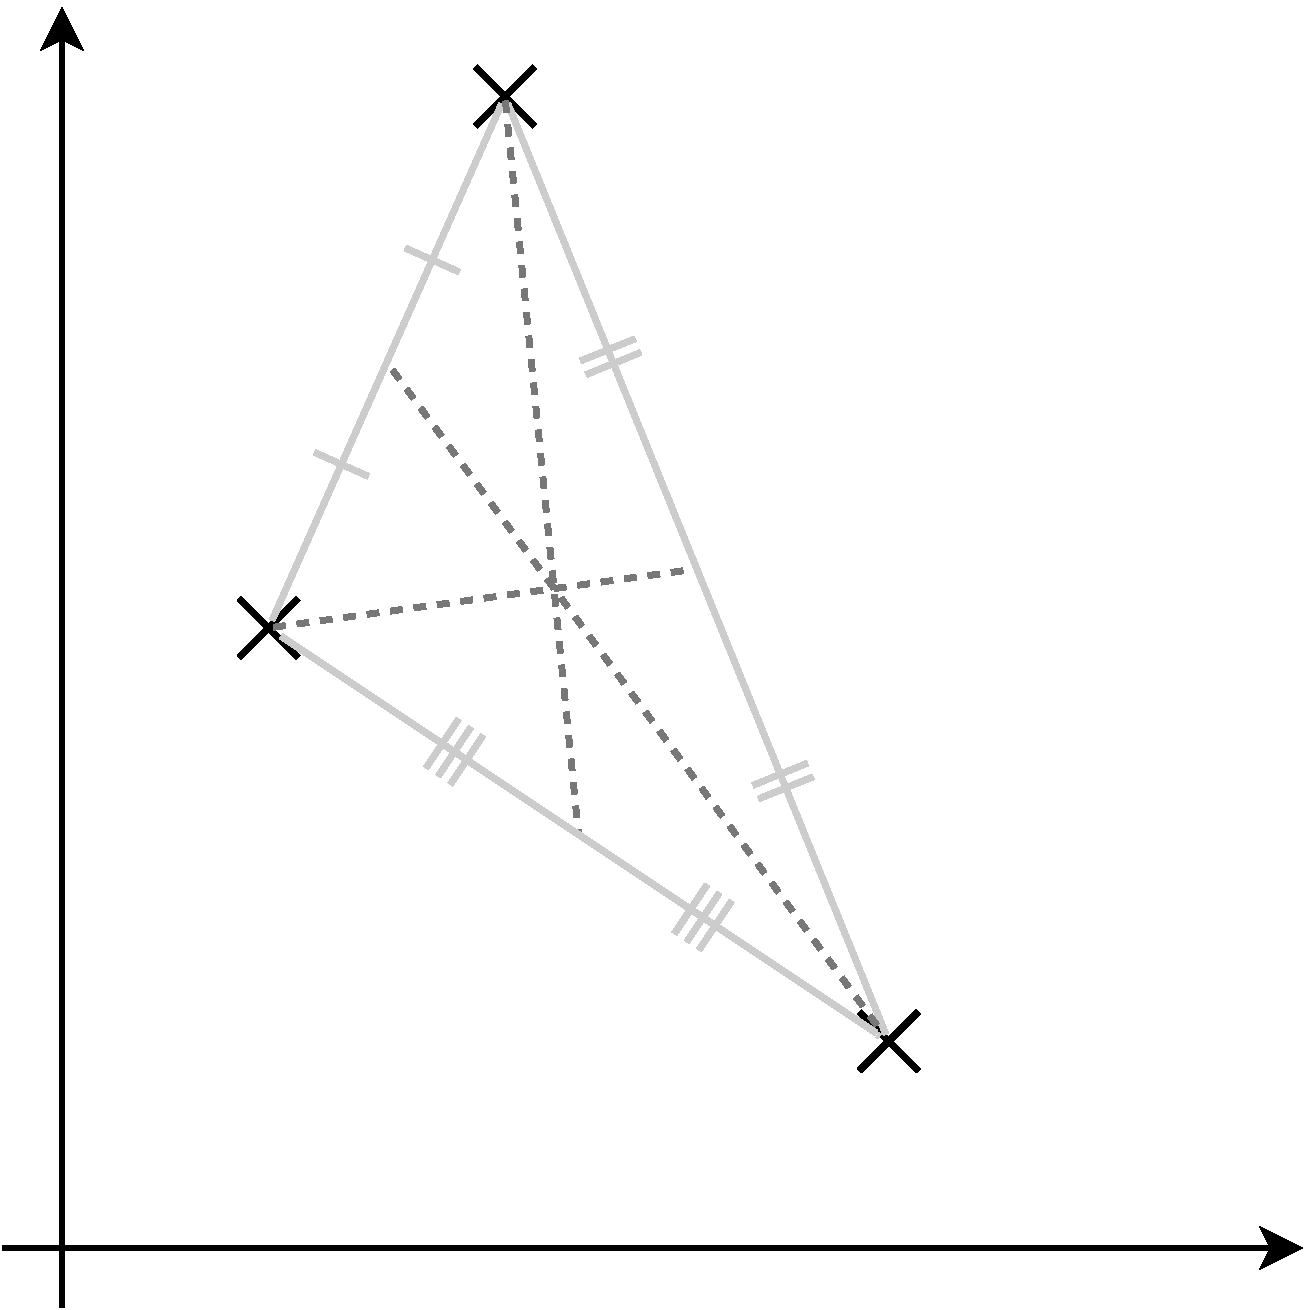
\includegraphics[width=0.5\textwidth]{img/centroid.pdf}
\caption{Centroid for three points in a 2 dimensional feature space}\label{fig:centroid}
\end{figure}

Equation~\ref{eq:sce} shows how the centroid ($C$) can be generated in a high-dimensional feature 
space (of $D$ dimensions), this works by taking the mean (Equation~\ref{eq:mean}) of each feature 
in the set of paintings ($x_1, x_2,\dotsc,x_k$) for a single year, this will give the point in 
feature space that is most central. This is the same technique used to generate centroids in most 
clustering algorithms ($k$-Means Clustering, for example).

\begin{equation}
\label{eq:sce}
\forall_{d \in D}\;C_d = \frac{1}{k}\sum^{k}_{i=1}{x_{i_{d}}}
\end{equation}

This may become a long operation depending on how many dimensions the feature space has. A
technique like \gls{pca}\cite{Jolliffe2002Principal} may be useful to help cut down the number of dimensions needed that this
algorithm uses.

Initially, as I wasn't producing histogram results from analysis techniques, this was a little
complex to do; each analysis technique had to have its own method of generating the centroid and
returning the data for this centroid. The change to histogram results made everything a lot easier
and, combined with the mean method from numpy, which can handle the mean along 
different axes, rather than just over a flattened array made this process a lot easier to compute,
especially as histograms from \gls{cv2} are returned as numpy arrays and the data passed into the centroid method is now an 
array of these histograms. Calculating the mean across the first axis has the effect of 
calculating the centroid. Equation~\ref{eq:mean-matricies} shows this mathematically on 2D 
Matrices where $\bar{x}_n$ is the mathematical mean of $x$ along axis $n$.

\begin{align}
x=&\begin{bmatrix}
\begin{bmatrix}
1.0 & 1.0 & 0.0 \\
0.0 & 1.0 & 1.0 \\
0.0 & 0.4 & 0.0 \\
\end{bmatrix} & 
\begin{bmatrix}
0.0 & 1.0 & 0.0 \\
1.0 & 1.0 & 1.0 \\
0.6 & 0.0 & 1.0 \\
\end{bmatrix}
\end{bmatrix} \nonumber \\
\bar{x}_1 =& 
\begin{bmatrix}
0.5 & 1.0 & 0.0 \\
0.5 & 1.0 & 1.0 \\
0.3 & 0.2 & 0.5 \\
\end{bmatrix}
\label{eq:mean-matricies}
\end{align}

Whilst the mean histogram could be a useful centroid, it doesn't fit with the idea of an artistic 
exemplar, it is quite possible that the art historians would be able to imagine a theoretical
painting which suits that year but they were limited to real paintings so it should follow that
the statistical methods are also be constrained in the same fashion.

A note on terminology; an \emph{artistic exemplar} is an exemplar which the art historians view
to be the most representative painting. A \emph{centroid} is the mean of a set of analysis over a
particular year and is a point in feature space, it is not an exemplar as it does not exists as a 
real painting. A \emph{statistical exemplar} is the nearest real painting to a centroid.

Statistical exemplars are generating by applying a nearest neighbour algorithm to all paintings
where the only neighbour is the centroid. This could be seen as a form of generalisation and may
help prevent overfitting of a classification technique. It may also show which years in which
the artistic exemplar commonly matches the statistical exemplars and where they do not. This gives
a vision of the difference between artistic and statistic exemplars and, perhaps, where the 
artistic exemplars are the outliers of a particular year.

%This could be seen as a form of generalisation. Though this may affect the results for the worse
%it may help prevent overfitting of the classification technique. It also shows which years are 
%commonly chosen as exemplars correctly and incorrectly, this should give a vision of the 
%difference between the artistic and statistic exemplars and where the artistic exemplars are the
%outliers of that particular year.

%To do this a Nearest Neighbour algorithm is applied to the data for that year from the centroid,
%this, of course, has the effect of picking the painting closest to the centroid, which is then
%used as the exemplar for that year. The same technique used to classify using artistic exemplars
%is then applied, only with these exemplars rather than the ones loaded from the exemplar file.

By re-using methods from the nearest-exemplar classifier (which uses the artistic exemplars only), 
the option to use inheritance to cut down on code repetition was made available by extending this
existing classifier and overriding the method which loaded the statistical exemplars from the 
\gls{csv} file to generate the centroids and statistical exemplars instead. Here the use of super 
calls in Python was confusing to a certain extent; listing~\ref{lst:py-super} shows one correct 
solution to this\footnote{There are, of course, other correct methods, but the one listed is one 
of the better solutions}.

\begin{lstlisting}[language=python, breaklines=true, label=lst:py-super, 
caption={Super method calls in Python}, frame=single]
# Note Base has to extend 'object' for super calls to work
class Base(object):
    def call(self, params):
        # ...

class Sub(Base):
    def call(self, params):
        # Before Base.call
        super(self, Sub).call(params)
        # After Base.call
\end{lstlisting}


\section{Filtering}
One area that was experimented with was the ability to filter paintings by certain pieces of 
metadata for that painting. Typically with would allow the filtering of just a single type of
painting (e.g. filtering out any painting which isn't a landscape to remove potential outliers).

Unfortunately, with most techniques this produces worst Correlation than not filtering by type,
this may be due to the limited size of the data-set. Removing the non-landscape 
paintings leaves such a gap in the years that $k$-Nearest Neighbour cannot classify the painting
correctly. Before filtering the data-set only contained 325 paintings, after filtering down to just
landscapes this was further reduced to 247 paintings.

A potential way of helping with this (and effectively filtering the data in a slightly different
fashion) is to round the year ($y$) of a painting to the nearest 5 years ($y_{_{5}}$). The maths 
to do this is shown in Equation~\ref{5-years}. 

\begin{equation}\label{5-years}
y_{_{5}} = 5\left\lfloor\frac{y}{5} \right\rfloor
\end{equation}

This does improve the correlation by a little as it helps to counteract the sparseness of the data
in the dataset. Whilst the improvements in correlation are nice, the information lost by rounding
is not really gained back by this increase in correlation.
